\documentclass[unicode,a4paper,11pt]{ltjsarticle}

\usepackage{luatexja-fontspec}
\setmainfont{TeX Gyre Termes}
% \setmainjfont[BoldFont = IPAGothic]{IPAMincho}
\setmathrm{Latin Modern Roman}
\setmainjfont{Noto Sans JP}

% ---Display \subsubsection at the Index
% \setcounter{tocdepth}{3}

% ---Setting about the geometry of the document----
% \usepackage{a4wide}
% \pagestyle{empty}

% ---Physics and Math Packages---
\usepackage{amssymb,amsfonts,amsthm,mathtools}
\usepackage{physics,braket,bm}

% ---underline---
\usepackage[normalem]{ulem}

% ---cancel---
\usepackage{cancel}

% --- surround the texts or equations
% \usepackage{fancybox,ascmac}

% ---settings of theorem environment---
% \usepackage{amsthm}
% \theoremstyle{definition}

% ---settings of proof environment---
% \renewcommand{\proofname}{\textbf{証明}}
% \renewcommand{\qedsymbol}{$\blacksquare$}

% ---Ignore the Warnings---
\usepackage{silence}
\WarningFilter{latexfont}{Some font shapes}
\WarningFilter{latexfont}{Font shape}
\WarningFilter{latexfont}{Size substitutions}
\ExplSyntaxOn
\msg_redirect_name:nnn{hooks}{generic-deprecated}{none}
\ExplSyntaxOff

% ---Insert the figure (If insert the `draft' at the option, the process becomes faster.)---
\usepackage{graphicx}
% \usepackage{subcaption}

% ----Add a link to a text---
\usepackage{url,hyperref}
\usepackage[dvipsnames,svgnames]{xcolor}
\hypersetup{colorlinks=true,citecolor=FireBrick,linkcolor=Navy,urlcolor=purple}
% ---refer `texdoc xcolor' at the command line---

% ---Tikz---
% \usepackage{tikz,pgf,pgfplots,circuitikz}
% \pgfplotsset{compat=1.15}
% \usetikzlibrary{intersections,arrows.meta,angles,calc,3d,decorations.pathmorphing}

% ---Add the section number to the equation, figure, and table number---
\makeatletter
   \renewcommand{\theequation}{\thesection.\arabic{equation}}
   \@addtoreset{equation}{section}
   
   \renewcommand{\thefigure}{\thesection.\arabic{figure}}
   \@addtoreset{figure}{section}
   
   \renewcommand{\thetable}{\thesection.\arabic{table}}
   \@addtoreset{table}{section}
\makeatother

% ---enumerate---
% \renewcommand{\labelenumi}{$\arabic{enumi}.$}
% \renewcommand{\labelenumii}{$(\arabic{enumii})$}

% ---Index---
% \usepackage{makeidx}
% \makeindex 

% ---Fonts---
% \renewcommand{\familydefault}{\sfdefault}

% ---Title---
\title{
    2024年度\ 春の学校\ しおり\ v2
}
\author{
  校長:宮根
}
\date{最終更新:\today}

\begin{document}

\maketitle

* This document is the spring school handbook. The English version begins from page \pageref{eng_page}.

\tableofcontents



\clearpage

\section{スケジュール}

\begin{center}
      \begin{tabular}{cll}\hline
            日        & 時間                 & 予定                                      \\ \hline
            4/6\ (土) & 13:00                & セミナーハウス到着                        \\
                      &                      & 荷物を部屋において、ゼミ室へ。            \\
                      & 13:20                & 発表開始                                  \\
                      & 16:30                & 発表終了                                  \\
                      &                      & 入浴など。                                \\
                      & 18:00\ $\sim$\ 19:00 & 夕食                                      \\
                      & 19:00\ $\sim$\ 22:00 & お茶会                                    \\
                      &                      & (片づけを含めた時間)                      \\
                      & 23:00                & 就寝                                      \\ \hline
            4/7\ (日) & 7:00                 & 起床                                      \\
                      & 7:30\ $\sim$\  8:30  & 朝食                                      \\
                      & 9:00                 & チェックアウト\ \&\ 発表開始              \\
                      & 11:40                & 発表終了                                  \\
                      &                      & お茶会・写真撮影など\ $\rightarrow$\ 解散 \\ \hline
      \end{tabular}
\end{center}

\begin{itemize}
      \item
            入浴ができるのは16:00\ $\sim$\ 22:00です。
      \item
            食事は上記の時間内に済ませてください。
      \item
            一応、チェックアウトは10:00までです。
      \item
            去年は(買い出し班が)少し早めに到着したら怒られました。
\end{itemize}

\section{発表タイムテーブル}

\begin{center}
      \begin{tabular}{clcl}\hline
            日        & 時間                  & 発表時間\ (分) & 発表者             \\ \hline
            4/6\ (土) & 13:20\ $\sim$\ 13:45  & 25             & 中里 弘道\ (教授)  \\
                      & 13:50\ $\sim$\ 14:00  & 10             & 落合 誠\ (助教)    \\
                      & 14:00\ $\sim$\ 14:10  &                & (10分\ 休憩)       \\
                      & 14:10\ $\sim$\ 14:20  & 10             & 渡辺 あかね\ (D)   \\
                      & 14:25\ $\sim$\ 14:35  & 10             & 岩村 海飛\ (D)     \\
                      & 14:40\ $\sim$\ 14:50  & 10             & 徳永 尚文\ (D)     \\
                      & 14:50\ $\sim$\ 15:05  &                & (15分\ 休憩)       \\
                      & 15:05\ $\sim$\ 15:45  & 40             & 谷口 永希\ (M2)    \\
                      & 15:50\ $\sim$\ 16:30  & 40             & 小市 明勢\ (M2)    \\ \hline
            4/7\ (日) & 9:00\ $\sim$\ 9:25    & 25             & 安倍 博之\ (教授)  \\
                      & 9:30\ $\sim$\ 10:10   & 40             & 永井 駿平\ (M2)    \\
                      & 10:10\ $\sim$\ 10:25  &                & (15分\ 休憩)       \\
                      & 10:25\ $\sim$\ 10:35  & 10             & 芝山 駿介\ (M1)    \\
                      & 10:40\ $\sim$\ 10:50  & 10             & 嶋田 直希\ (M1)    \\
                      & 10:55\ $\sim$\ 11:05  & 10             & 宮根 一樹\ (M1)    \\
                      & 11:10\ $\sim$\ 111:40 & 30             & Raiyan Haque\ (B4) \\ \hline
      \end{tabular}
\end{center}

\begin{itemize}
      \item
            発表時間は\textbf{質疑応答込み}の時間です。タイムキーピングをお願いします。
\end{itemize}

\section{部屋割り}

\begin{center}
      \begin{tabular}{cl}\hline
            部屋番号 & メンバー                                      \\ \hline
            301      & 中里 弘道                                     \\
            302      & 安倍 博之                                     \\
            303      & 渡辺 あかね                                   \\
            202      & 岩村 海飛、徳永 尚文、落合 誠                 \\
            203      & 小市 明勢、谷口 永希、永井 駿平、芝山 駿介    \\
            204      & 嶋田 直希、佐久間 紀丞、下田 幹人、堀内 嵩真  \\
            205      & 宮根 一樹、花村 晃、吉田 聡一郎、Raiyan Haque \\ \hline
      \end{tabular}
\end{center}

\begin{itemize}
      \item
            従わなくて結構です。
      \item
            宿泊部屋での飲酒は禁止だそうです。
\end{itemize}


\section{電車利用の際の参考経路}

\vspace*{5pt}

\begin{center}
      \begin{minipage}[ht]{0.48\columnwidth}
            \textbf{通常班}

            \vspace*{5pt}

            \begin{tabular}{cl}\hline
                  時間     &                                 \\ \hline
                  9:55 発  & 高田馬場                        \\
                           & $\downarrow$\ JR\ 山手線        \\
                  10:20 着 & 品川                            \\
                  10:34 発 &                                 \\
                           & $\downarrow$\ JR\ こだま\ 717号 \\
                  11:12 着 & 熱海                            \\
                  11:32 発 &                                 \\
                           & $\downarrow$\ JR\ 伊東線        \\
                  12:05 着 & 川奈                            \\ \hline
            \end{tabular}
      \end{minipage}
      \begin{minipage}[ht]{0.48\columnwidth}
            \textbf{買い出し班}

            \vspace*{5pt}

            \begin{tabular}{cl}\hline
                  時間     &                                 \\ \hline
                  8:54 発  & 高田馬場                        \\
                           & $\downarrow$\ JR\ 山手線        \\
                  9:18 着  & 品川                            \\
                  9:34 発  &                                 \\
                           & $\downarrow$\ JR\ こだま\ 717号 \\
                  10:10 着 & 熱海                            \\
                  10:45 発 &                                 \\
                           & $\downarrow$\ JR\ 伊東線        \\
                  11:16 着 & 川奈                            \\ \hline
            \end{tabular}
      \end{minipage}
\end{center}

\begin{itemize}
      \item
            料金はいずれも4,410円(乗車券$+$自由席特急券)です。\\
            このルートに従う必要はありませんが、さすがに熱海あたりからは一緒になると思います。
      \item
            (特急を除けば、)買い出し班と通常班の間には電車がありません。
      \item
            通常班も熱海11:32発の電車を逃したら、次は12:24発になります。
      \item
            去年は電子マネーもOKでした。後で、確認します。
      \item
            帰りに新幹線の指定席を買う方は、終了時刻の前後があるため注意してください。
      \item
            買い出し班は川奈駅で徳永さんと合流して、そのまま隣にある東急ストアでお買い物です。
\end{itemize}


\section{その他・注意事項}

\subsection*{経費関連}

\begin{itemize}
      \item
            交通費と食費は後で支払われます。交通費の支給額は(可能であれば)後で載せておきます。
      \item
            食費は朝$+$夕で1,980円、お茶会代1,020円、合わせて3,000円を集めます。\\
            余ったお茶会代はどうするか誰かと後で相談します。
      \item
            宿泊費は(一部の方は除いて)実験実習費から支払われるそうです。
\end{itemize}

\subsection*{持ち物}

\begin{itemize}
      \item
            タオル
      \item
            歯ブラシ・歯磨き粉
      \item
            洗顔道具
      \item
            着替え・寝間着
      \item
            ドライヤー(?)
      \item
            マルチタップ(部屋の人が喜びます)
      \item
            ウノ!(など。校長が喜びます!)
\end{itemize}

その他

\begin{itemize}
      \item
            シャンプー、ボディーソープはあるそうです。
      \item
            研究室から指示棒とレーザーポインタを持っていきます。
      \item
            徳永さんがクーラーボックスを持ってきてくださるようです。ありがとうございます。
\end{itemize}

\subsection*{買い物リスト}

(更新中)

\subsection*{その他の連絡事項}

\begin{itemize}
      \item
            徒歩20分のところにファミマがあります。
      \item
            パソコンとプロジェクターで発表可。
      \item
            20:00以降の外出は控えてください。
      \item
            Wifiは宿泊部屋、ゼミ室、食堂にあり。
      \item
            冷蔵庫は各宿泊部屋にあり。
      \item
            お茶会用に食堂を借りるときは校長が交渉しておきます。
\end{itemize}


\section{リンク集 / Links}

\begin{itemize}
      \item
            \href{https://www.waseda.jp/inst/student/facility/seminar/facility/izukawana}{ホームページ / Webpage}
      \item
            \href{https://www.waseda.jp/inst/student/facility/seminar/flow/tips}{利用上の心得 / Usage tips}
\end{itemize}


\section{懇親会 / Konshinkai}

こんなのが引継ぎのフォルダにありました。

I found the following in the shared folder.

\begin{center}
      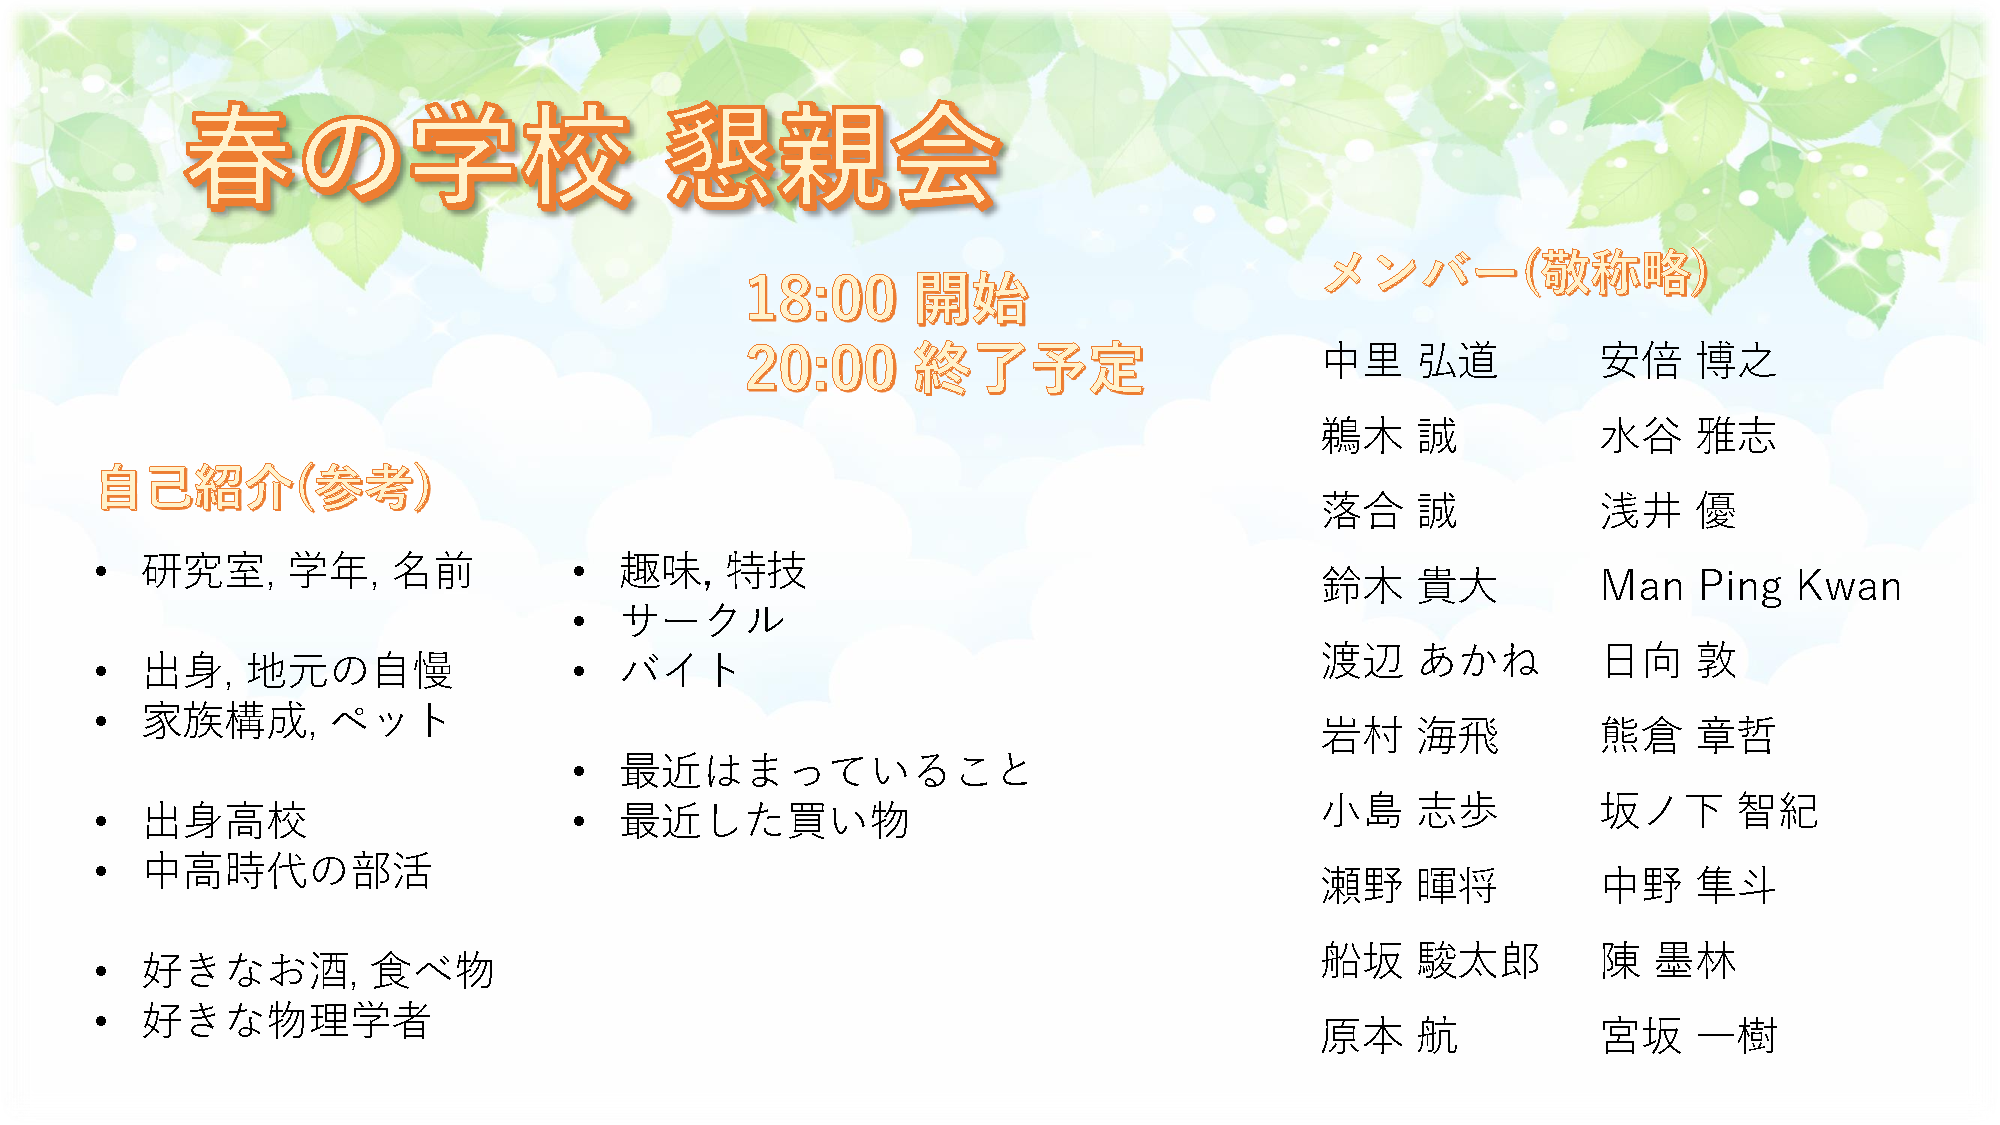
\includegraphics[width=1.0\linewidth]{konshinkai.pdf}
\end{center}


\clearpage

\setcounter{section}{0}

Here is the English version. Since I spent a lot of time making this version, I hope some English students to read this eagerly.

\label{eng_page}

\section{Schedule}

\begin{center}
      \begin{tabular}{cll}\hline
            Date          & Time               & Schedule                                           \\ \hline
            Sat. Apr. 6th & 1:00 p.m.          & Arrive at seminar house                            \\
                          &                    & Put loads in the room and move to the seminar room \\
                          & 1:20               & Start presentation                                 \\
                          & 4:30               & End                                                \\
                          &                    & bathe, etc.                                        \\
                          & 6:00  $\sim$ 7:00  & Dinner                                             \\
                          & 7:00  $\sim$ 10:00 & Party                                              \\
                          &                    & (Clean up by 10:00 p.m.)                           \\
                          & 11:00 p.m.         & Go to bed                                          \\ \hline
            Sun. Apr. 7th & 7:00 a.m.          & Get up                                             \\
                          & 7:30 $\sim$  8:30  & Breakfast                                          \\
                          & 9:00               & Complete check out\ \&\ Start presentation         \\
                          & 11:40 a.m.         & End                                                \\
                          &                    & Tea time, Photo, etc.\ $\rightarrow$\ Breakup!     \\ \hline
      \end{tabular}
\end{center}

\begin{itemize}
      \item
            Bathing is from  4:00 p.m. to 10:00 p.m.
      \item
            Meals should be finished by the time mentioned above.
      \item
            Checkout is by 10:00 a.m.
      \item
            In the last year, we made the director of the seminar house angry since some students arrived earlier.
\end{itemize}

\clearpage

\section{Timetable}

\begin{center}
      \begin{tabular}{clcl}\hline
            Date          & Time                       & Duration\ (min) & Presenter                        \\ \hline
            Sat. Apr. 6th & 1:20 p.m.\ $\sim$\ 1:45    & 25              & Hiromichi Nakazato\ (Professor)  \\
                          & 1:50\ $\sim$\ 2:00         & 10              & Makoto Ochiai\ (Assistant Prof.) \\
                          & 2:00\ $\sim$\ 2:10         &                 & (10 min break)                   \\
                          & 2:10\ $\sim$\ 2:20         & 10              & Akane Watanabe\ (D)              \\
                          & 2:25\ $\sim$\ 2:35         & 10              & Kaito Iwamura\ (D)               \\
                          & 2:40\ $\sim$\ 2:50         & 10              & Takafumi Tokunaga\ (D)           \\
                          & 2:50\ $\sim$\ 3:05         &                 & (15 min break)                   \\
                          & 3:05\ $\sim$\ 3:45         & 40              & Eiki Taniguchi\ (M2)             \\
                          & 3:50\ $\sim$\ 4:30 p.m.    & 40              & Akinari Koichi\ (M2)             \\ \hline
            Sun. Apr. 7th & 9:00 a.m \ $\sim$\ 9:25    & 25              & Hiroyuki Abe\ (Professor)        \\
                          & 9:30\ $\sim$\ 10:10        & 40              & Shunpei Nagai\ (M2)              \\
                          & 10:10\ $\sim$\ 10:25       &                 & (15 min break)                   \\
                          & 10:25\ $\sim$\ 10:35       & 10              & Shunsuke Shibayama\ (M1)         \\
                          & 10:40\ $\sim$\ 10:50       & 10              & Naoki Shimada\ (M1)              \\
                          & 10:55\ $\sim$\ 11:05       & 10              & Itsuki Miyane\ (M1)              \\
                          & 11:10\ $\sim$\ 111:40 a.m. & 30              & Raiyan Haque\ (B4)               \\ \hline
      \end{tabular}
\end{center}

\begin{itemize}
      \item
            Presentation time includes Q\&A sessions. Please be careful \textit{not} to extend.
\end{itemize}

\section{Room Allocation}

\begin{center}
      \begin{tabular}{cl}\hline
            Room Number & Member                                                            \\ \hline
            301         & Hiromichi Nakazato                                                \\
            302         & Hiroyuki Abe                                                      \\
            303         & Akane Watanabe                                                    \\
            202         & Kaito Iwamura, Takafumi Tokunaga, Makoto Ochiai                   \\
            203         & Akinari Koichi, Eiki Taniguchi, Shunpei Nagai, Shunsuke Shibayama \\
            204         & Naoki Shimada, Kisuke Sakuma, Mikito Shimoda, Shuma Horiuchi      \\
            205         & Itsuki Miyane, Akira Hanamura, Soichiro Yoshida, Raiyan Haque     \\ \hline
      \end{tabular}
\end{center}

\begin{itemize}
      \item
            You don't need to follow the table above.
      \item
            It is \textit{not} permitted to drink alcohol in the room.
\end{itemize}


\section{Examples of Transfers}

\vspace*{5pt}

\begin{center}
      \begin{minipage}[ht]{0.48\columnwidth}
            \textbf{Normal Team}

            \vspace*{5pt}

            \begin{tabular}{cl}\hline
                  Time           &                                 \\ \hline
                  From 9:55 a.m. & Takadanobaba                    \\
                                 & $\downarrow$\ JR\ Yamanote line \\
                  To 10:20       & Shinagawa                       \\
                  From 10:34     &                                 \\
                                 & $\downarrow$\ JR\ Kodama\ 717   \\
                  To 11:12       & Atami                           \\
                  From 11:32     &                                 \\
                                 & $\downarrow$\ JR\ Ito line      \\
                  To 12:05       & Kawana                          \\ \hline
            \end{tabular}
      \end{minipage}
      \begin{minipage}[ht]{0.48\columnwidth}
            \textbf{Grocery Shopping Team}

            \vspace*{5pt}

            \begin{tabular}{cl}\hline
                  Time           &                                 \\ \hline
                  From 8:54 a.m. & Takadanobaba                    \\
                                 & $\downarrow$\ JR\ Yamanote line \\
                  To 9:18        & Shinagawa                       \\
                  From 9:34      &                                 \\
                                 & $\downarrow$\ JR\ Kodama\ 717   \\
                  To 10:10       & Atami                           \\
                  From 10:45     &                                 \\
                                 & $\downarrow$\ JR\ Ito line      \\
                  To 11:16       & Kawana                          \\ \hline
            \end{tabular}
      \end{minipage}
\end{center}

\begin{itemize}
      \item
            It costs 4,410 Yen for both courses. \\
            You don't need to follow the root mentioned above but, as I think, most people will join at the Atami station.
      \item
            There is no train between the normal team and the shopping team from Atami station. So we can't be late. I will try my best.
      \item
            By the way, if the normal team member misses the train from 11:32 a.m., he or she has to take the train from 12:24 p.m. There are fewer trains in Shizuoka than in Tokyo.
      \item
            As I remember, we could pay by IC. I will confirm and announce it later.
      \item
            When you buy a reserved seat on the Shinkansen for a return trip, you should be careful since the seminar can extend. I recommend you buy a ticket just before taking the train.
      \item
            The member of the grocery shopping team should meet Tokunaga-san at the Kawana station and buy groceries at the Supermarket next to the station.
\end{itemize}


\section{Notes}


\subsection*{Money}

\begin{itemize}
      \item
            Transportation and food expenses will be paid later by the university. If I get to know the amount of money paid by the school, I will write here.
      \item
            I will gather 3,000 Yen from each member. The breakdown is 1,980 yen for breakfast and dinner and 1,020 yen for the party. Do not give anything other than Japanese yen.
      \item
            The accommodation fee has already been paid. So, you shouldn't care about it.
\end{itemize}


\subsection*{Belongings}

\begin{itemize}
      \item
            Towel
      \item
            Toothbrush, Toothpaste
      \item
            Face-washing Tools
      \item
            Change of clothes and nightclothes
      \item
            Dryer
      \item
            Power strip (Your roommate will be pleased.)
      \item
            UNO! (etc. Kocho will be pleased.)
      \item
            Funny stories (Everyone will be pleased.)
\end{itemize}

Others:
\begin{itemize}
      \item
            There seems to be shampoo and body soap.
      \item
            Kocho should bring indicator sticks and laser pointers from the Lab.
      \item
            Tokunaga-san brings the cooler-box. Thank you very much.
\end{itemize}


\subsection*{Shopping List}

(updating $\cdots$)


\subsection*{Other notifications}

\begin{itemize}
      \item
            There is a convenience store a 20-minute walk away from the seminar house.
      \item
            PC and projector are available.
      \item
            Please do not go out from 8:00 p.m.
      \item
            Wi-Fi is available in accommodation rooms, seminar rooms, and dining rooms.
      \item
            There are refrigerators in each accommodation room.
      \item
            Kocho should negotiate whether the dining room can be used for the banquet.
\end{itemize}

\end{document}
